% ============================================================
% PHẦN Faster-GS (bản 45 phút, rút gọn) — 2 slide
% Rút gọn từ part_fastergs_01.tex..08.tex (bản full, ../part_fastergs_*.tex)
% ============================================================

% --- Slide A ---
\begin{frame}{Faster-GS (CVPR 2026): 4 cơ chế mới luôn bật}
\footnotesize
\begin{itemize}
    \item \textbf{Fused Adam}: 1 kernel CUDA elementwise, đúng công thức Adam chuẩn (không đổi thuật toán, chỉ giảm overhead kernel-launch).
    \item \textbf{3D anti-aliasing filter}: clamp scale tối thiểu theo khoảng cách camera $\Rightarrow$ chống alias.
    \item \textbf{Morton Z-order reordering}: sắp Gaussian theo mã bit-interleave (mỗi 5000 iteration) $\Rightarrow$ tăng cache locality cho rasterizer.
    \item \textbf{Random-init fallback}: sample đều trong hình cầu bằng $r=R\cdot u^{1/3}$ khi COLMAP thiếu \texttt{points3D}.
    \item[$\Rightarrow$] Cả 4 đều \textbf{luôn bật}, không còn cờ toggle.
    \item \textit{Ngoại lệ}: MCMC densification có sẵn trong code nhưng \textbf{giữ tắt} — xung đột kiến trúc với densify chính của FastGS.
\end{itemize}
\centering
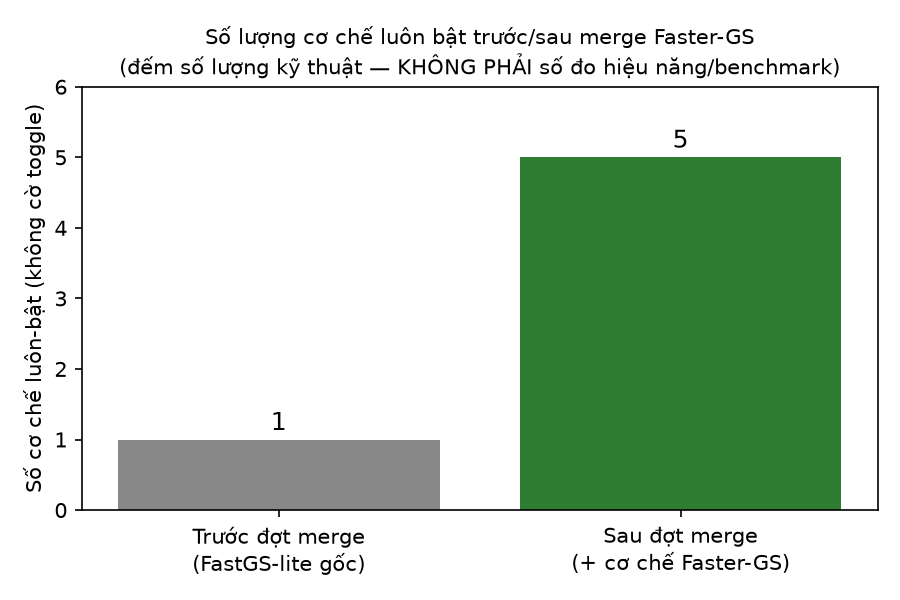
\includegraphics[width=0.3\linewidth]{../../BOOK/fastergs_merge_figures/00_techniques_overview.png}
\captionof{figure}{\footnotesize Số cơ chế luôn bật trước/sau đợt merge (đếm số lượng, không phải benchmark)}
\end{frame}

% --- Slide B ---
\begin{frame}{Bug đã sửa: \texttt{opacity\_reset\_interval} không co giãn theo iterations}
\footnotesize
\begin{itemize}
    \item \textbf{Nguyên nhân thật} của các điểm sụt Score đã thấy (Slide 33--37): \texttt{opacity\_reset\_interval} hardcode \textbf{3000} (đúng cho lịch gốc 30k), \textbf{không co giãn} theo \texttt{iterations} đã rút ngắn $\Rightarrow$ reset kích hoạt quá sớm.
    \item Bằng chứng thật: PSNR rơi \textbf{22.02$\to$5.92} tại iteration 3000 (scene HCM0539).
    \item \textbf{Cách sửa}: field mới \texttt{opacity\_reset\_frac=0.2}, co giãn \texttt{opacity\_reset\_interval = round(0.2$\times$iterations)}.
    \item Chưa có log thật "sau khi sửa" — chưa build/chạy lại (không có GPU ở môi trường phát triển).
\end{itemize}
\centering
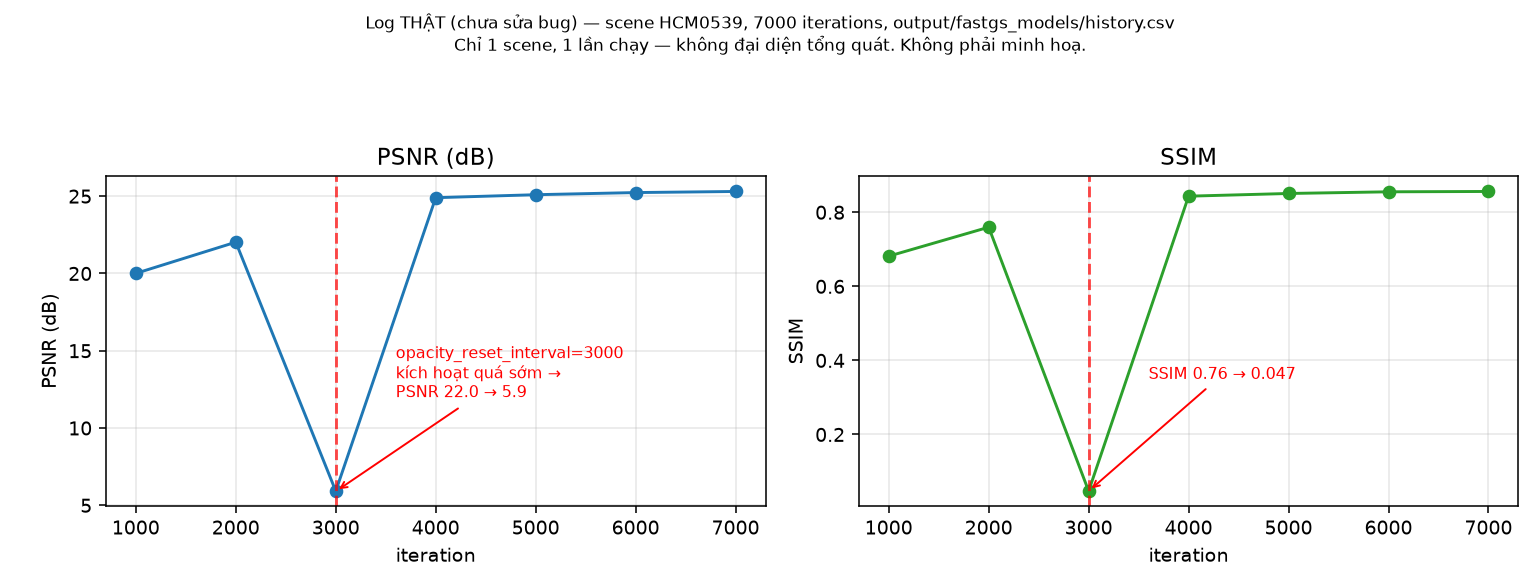
\includegraphics[width=0.32\linewidth]{../../BOOK/adc_figures/12_opacity_reset_crash_real_log.png}
\captionof{figure}{\footnotesize Log thật (trước khi sửa): PSNR sụp tại iteration 3000}
\end{frame}
